\chapter{Literature Review}

\section{Sanitization}
Sanitization is the process of removing sensitive information from a document or other message or sometimes encrypting messages, so that the document may be distributed to a broader audience. Sometimes sanitization can be called as an operation that ensures that user input can be safely used in an SQL query. Web applications use malicious input as part of a sensitive operation without having properly checked or sanitized the input values from the user. Previous research on vulneribility analysis has mostly focused on identifying cases which web applications directly uses external input for critical operations. It is suggested that always use proper sanitization method to validate external input values from the user for any application.For example, user inputs must always flow through a sanitizing function before flowing into a SQL query or HTML, to avoid SQL injection or cross-site scripting vulnerabilities.\\

Reflection of security breaches are very significant for high assurance system. For examples of this type of systems are aircraft navigation, where a fault could lead to a crash, various control systems which has critical infrastructure , where an error 
could cause toxic waste to leak, and weapons targeting, where an inaccuracy could result in severe collateral damage. In such
operational environments, the impact is virtually irreversible and must therefore be prevented even if it is likely to occur
with low probability.It's always good that transforming information to a form which is suitable for release or sanitize the information by redacting some portions of it.\\

Three of the top five most common website attacks are SQL injection, cross-site scripting (XSS), and remote file inclusion (RFI). The root cause of these attacks is common: input sanitization. All three exploits are leveraged by data sent to the web server by the end user. When the end user is a good guy, the data he sends the server is relevant to his interaction with the website. But when the end user is a hacker, he/she can exploit this mechanism to send the web server input which is deliberately constructed to escape the legitimate context and execute unauthorized actions.\\

Input sanitization describes cleansing and scrubbing user input to prevent it from jumping the fence and exploiting security holes. But thorough input sanitization is hard. While some vulnerable sites simply don't sanitize at all, others do so incompletely, lending their owners a false sense of security.\\

Some basic purpose of sanitization are given below:
\begin{itemize}
	\item Remove malicious elements from the input.
	\item To identify the set of parameters and global variables which must be sanitized before calling functions.
	\item It is acceptable to first pass the untrusted user input through a trusted sanitization function.	
	\item Any user input data must flow through a sanitization function before it flows into a SQL query.
	\item Confidential data needs to be cleansed to avoid information leaks.
	\item Most paths that go from a source to a sink pass through a sanitizer.
	\item Developers typically define a small number of sanitization functions in libraries.
	\item Prevent web attacks using input sanitization.
\end{itemize}

\section{Declassification}
Information security has a challenge to address: enabling information flow controls with expressive information release (or declassification) policies. In a scenario of systems that operate on data with different sensitivity levels, the goal is to provide security assurance via restricting the information flow within the system. Practical security-typed languages support some form of declassification through which high-security information is allowed to flow to a low-security system or observer.\\

United States Federal Trade Commission reveals the damage that is continually caused by electronic information leakage. In protecting sensitive information, including everything from credit card information to military secrets to personal, medical information, there is a highly
need for software applications with strong, confidentiality guarantees.
Security-typed languages promise to be a valuable tool in making provably secure software applications. In such languages, each
data item is labeled with its security policy. In practical security-typed languages support some form of declassification, in which high-security information is permitted to flow to a low-security receiver/observer \\

To declassify information means lowering the security classification of selected information. Sabelfeld and Sands \cite{ref_3_sabelfeld2009declassification} identify four different dimensions of declassification, what is declassified, who is able to declassify, where the declassification occurs and when the declassification takes place.\\

Myers and Liskov introduced the decentralized label model \cite{ref_4_myers2000protecting}, describing how labels could be applied
to a programming language and then used to check information
flow policy compliance in distributed systems. The framework
includes a declassify function for downgrading data if the
owners policies allow. The model allows principals to define their own downgrading policies.\\

\textbf{Dimensions of declassification:}
Classification of the basic declassification goals according to four axes: what information is released, who releases information, where in the system information is released and when information can be released.

\begin{itemize}
   \item What: Selective or Partial information flow policies \cite{ref_5_cohen1977information,ref_6_cohen1978information,ref_7_joshi2000semantic,ref_8_giacobazzi2005adjoining} regulate what
   information may be released. Partial release guarantees that only a part of a secret is
   released to a public domain. Partial release can be specified in terms of precisely which
   parts of the secret are released. This is useful,
   for example, when partial information about a credit card number or a social security number is used for logging.
   
   \item Who: In a computing system it is essential to specify who controls information release .
   Ignoring the issue of control opens up attacks where the attacker hijacks release
   mechanisms to launder secret information. Myers and Liskov decentralised label
   model \cite{ref_9_myers1997decentralized} security labels with explicit ownership information. According to this approach, information release of some data is safe if it is performed by the
   owner who is explicitly recorded in the data security label. This model has been used for enhancing Java with information flow controls \cite{ref_10_myers1999jflow} and has been implemented in
   the Jif compiler \cite{ref_11_myers2001jif}.
   
   \item Where: In a system information  Where is an important aspect of information release.One can ensure that no other  part can release further information.
   by delegating particular parts of the system to release information.Declassification
   via encryption is not harmful as long as the program is, in some sense, noninterfering
   before and after encryption.  A combination of \enquote{where} and \enquote{who} policies in the presence of encryption has
   been recently investigated by Hicks et al. \cite{ref_12_hicks2005declassification}
   
   \item When: The fourth dimension of declassification is  \enquote{when} information should be released.The work of Giambiagi and Dam \cite{ref_19_giambiagi2003secure} focuses on the correct implementation of security protocols. Here the goal is not to prove a noninterference property of the protocol, but to use the components of the protocol description as a specification of what and when information may be released.Chong and Myers security policies \cite{ref_13_chong2004security} address when information is released.By annotating variables this is achieved.
   
\end{itemize}

For a given model, the \enquote{what} and \enquote{when} dimensions seem relatively straightforward to define formally. The \enquote{what} dimension abstracts the extensional semantics
of the system; the \enquote{when} dimension can be distinguished from this since it requires an intensional semantics that (also) models time, either abstractly in terms of complexity
or via intermediate events in a computation. The \enquote{who} and \enquote{where} dimensions are
harder to formalize in a general way, beyond saying that they cannot be captured by the
\enquote{what} and \enquote{when} dimensions.

\section{Authentication}
Authentication is the mechanism which confirms the identity of users trying to access a system. For a user to be granted access to a resource, they must first prove that they are who they claim to be. Generally this is handled by passing a key with each request (often called an access token, User verification using user id and password). The system or server verifies that the access token or user id and password is genuine, that the user does indeed have the required privileges to access the requested resource and only then the request granted.\\
Also authentication can be defined as it is the process by which the system validates a user's logon information. A user's name and password are compared to an authorized list and if the system detects a match then access is granted to the extent specified in the permission list for that user.\\

One familiar use of authentication and authorization is access control. A computer system that is supposed to be used only by those authorized must attempt to detect and exclude the unauthorized. Common examples of access control involving authentication include:
\begin{itemize}	
	\item A computer program using a blind credential to authenticate to another program.
	\item Logging in to a computer.	
	\item Using an Internet banking system.
	\item Withdrawing cash from an ATM and more
	\item Assurance of identity of person or originator of data.
\end{itemize}

 A variety of authentication technologies have hit the market over the years.To better understand what they are and how they compare to the user name/password combination, it helps to be familiar with the standard authentication factors something you know, something you have and something you are and how each technology leverages them to power its authentication capabilities.
 \begin{itemize}	
	\item Something you know is a bit of knowledge committed to memory, such as a password or
	 an answer to a secret question.
	\item Something you have is an item that is owned or carried, such as a smart card or similar
	 hardware device.
	\item	 Something you are is a physical attribute that can be identified, such as a fingerprint or voice.
\end{itemize}

According to the networkworld \cite{ref_21_networld} now-a-days seven strong authentication methods are:
\begin{itemize}
\item Computer recognition software.
\item Biometrics
\item E-mail or SMS one-time password (OTP).
\item One Time Password (OTP) token.
\item Out of band.
\item Peripheral device recognition.
\item Scratch-off card.
\end{itemize}	


\section{ Detecting Information Flow Errors During Design}
If a step of function call like authentication, sanitization or declassification is missing inside the program then this can lead to software vulnerabilities. In the figure \ref{figure_FunctionCallMissing} left side picture depicted that it has three functions. Among them func2() is named either sanitization/declassification/authentication function. Which means in this scenario there will be no error regarding sanitization/declassification/authentication function. On the other hand the right side picture represents there is a missing function of sanitization/declassification/authentication function. That's why it is the buggy path of UML state charts during design stage of software life cycle. 
\begin{figure}[htbp]
	\centering
	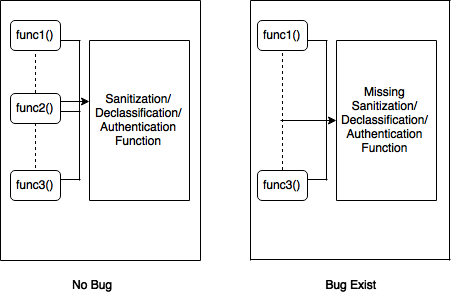
\includegraphics{styles/FunctionCallMissing.png}
	\caption{Information flow errors during design}
	\label{figure_FunctionCallMissing}
\end{figure}


\section{ Detecting Information Flow Errors During Coding}

Figure \ref{figure_bug_detection_during_coding} depicts two explicit information flows according to A lattice model of secure information flow of Denning \cite{ref_14_denning1976lattice} contained in two systems (system 1) and (system 2)
where each of the flows starts with statement variable a and ends with leaving the system. The the variable declaration up to outside the system represent C language statements. System 1 is depicted in left side containing the flow from the source to the sink and leaving the system indicated with circles at the top and bottom of each of the
two information flows. A source is any function or programming language statement which provides private information through a system boundary. A sink can be a function call or programming language statement which exposes private information to the outside of the system through a system boundary. A system boundary can be a statement, function call, class, package or module. In figure 2.2 the source and sink represent C language statements where information enters and respectively leaves system 1 or system 2. The variable a was tagged with label \enquote{H} (confidential) as it inserts confidential information into system 1. The arrows represent the passing of the confidential label \enquote{H} between the program statements. When a variable labeled with \enquote{H} is about to leave system 1 or system 2 without passing through either authentication/declassifiaction/sanitization function then a bug report should be created.In figure 2 right side system has a bug because it passes a secured/confidential information without passing through authentication/declassifiaction/sanitization function. These functions either authenticated,declassified or sanitized  secured/confidential information and makes the variable label as \enquote{L} to leave the system. But in the left part of the picture there is no bug as in this system, secured/confidential information and the variable which is labeled with \enquote{H} passes through either authentication/declassifiaction/sanitization function.

\begin{figure}[htbp]
	\centering
	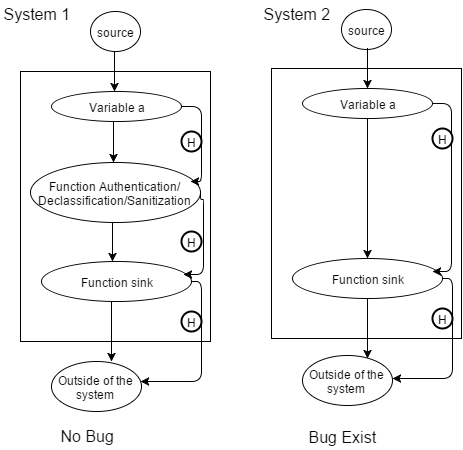
\includegraphics{styles/bug_detection_during_coding.png}
	\caption{Information flow errors during coding}
	\label{figure_bug_detection_during_coding}
\end{figure}
